% Copyright (c)  2005-2010 EDF-EADS-PHIMECA.
% Permission is granted to copy, distribute and/or modify this document
% under the terms of the GNU Free Documentation License, Version 1.2
% or any later version published by the Free Software Foundation;
% with no Invariant Sections, no Front-Cover Texts, and no Back-Cover
% Texts.  A copy of the license is included in the section entitled "GNU
% Free Documentation License".
\renewcommand{\filename}{docUC_StochProc_WhiteNoise.tex}
\renewcommand{\filetitle}{UC : Manipulation of a White Noise}

% \HeaderNNIILevel
 \HeaderIILevel
%\HeaderIIILevel



\index{Stochastic Process!White Noise}


This section details first how to create and manipulate a white noise.\\

A white noise $\underline{\epsilon}(\omega,t)$ is a stochastic process such that :
\begin{equation} \label{whiteNoiseDef}
\left\{
\begin{array}{l} 
  E[\underline{\epsilon}(\omega,t)]  = 0 \\
  Var[\underline{\epsilon}(\omega,t)]  = \sigma^2 < +\infty \\
 \forall  t \neq s , \, Cor[\underline{\epsilon}(\omega,s), \underline{\epsilon}(\omega,t)] = 0 \\
 (\underline{\epsilon}(\omega,t))_t \mbox{ are identically distributed}
\end{array} 
\right.
\end{equation}


Open TURNS proposes to model it through the object  \emph{WhiteNoise} defined by a time grid and a distribution with zero mean and finite standard deviation.\\

If the distribution has a mean different from zero, Open TURNS sends a message to prevent the User and does not allow the creation of such a WhiteNoise.\\
The $WhiteNoise$ object inherits from $Process$ object.
Thus, it is possible to get its marginal process, its time grid, its dimension and to get several realization at a time of the process.\\

Details on each object may be found in the User Manual  (\href{OpenTURNS_UserManual_TUI.pdf}{see User Manual - Stochastic Process}).\\

\requirements{
  \begin{description}
  \item[$\bullet$] a distribution : {\itshape $myDistribution$}
  \item[type:]  Distribution
  \end{description}

  \begin{description}
  \item[$\bullet$] a time grid : {\itshape $myTimeGrid$}
  \item[type:]  RegularGrid
  \end{description}

}
{
  \begin{description}
  \item[$\bullet$] a white noise {\itshape myWhiteNoise}
  \item[type:]  WhiteNoise
  \end{description}

  \begin{description}
  \item[$\bullet$] some graphs of trajectories versus time or in the phase space : {\itshape myGraph}
  \item[type:]  Graph
  \end{description}
}

\textspace\\
Python script for this UseCase :

\begin{lstlisting}
  # Creation of a white noise
  # From a distribution and a time grid
  myWhiteNoise = WhiteNoise(myDistribution, myTimeGrid)

  # Creation of a white noise
  # using a distribution and the default RegularGrid for time instants
  # care! This RegularGrid has one instant = 0
  myWhiteNoise = WhiteNoise(myDistribution)

  # Get a realization of the process
  realization = myWhiteNoise.getRealization()

  # Get a sample of N realizations of the process
  sample = myWhiteNoise.getSample(N)

  
  # For a White Noise of dimension d > 1 : 
  # Print one realization of both marginals $i$ anf $j$ in the phase space Xi versus Xj
  # from a process of dimension d 

  realisation = myWhiteNoise.getRealization()
  myGraph = Graph('2D White Noise - Marginals i and j', 'Xi', 'Xj', True)

  # get the values (of dimension d) of the realisation
  values = realisation.getNumericalSample()

  # get the values of marginals i anj
  marginalValues = values.getMarginal(Indices(i,j))

  # add the trajectory into the graph 
  myGraph.add(Curve(marginalValues))

  # For a White Noise of dimension d = 1 : 
  # Print one realization versus time
  realization = myWhiteNoise.getRealization()
  myGraph = realization.drawMarginal(0)
  
  # Get the i-th marginal of the process
  myMarginalWhiteNoise = myWhiteNoise.getMarginalProcess(i)

  # Get the marginal of index in (i,j,k) of the process   
  myIndices = Indices(i,j,k)
  myMarginalWhiteNoise = myWhiteNoise.getMarginalProcess(myIndices)

  # Get the distribution of the White Noise
  myWhiteNoiseDistribution = myWhiteNoise.getDistribution()

  # Set a new distribution for the White Noise
  myWhiteNoiseDistribution.setDistribution(newDistribution)

  # We make a graph using the TimeSeries draw marginal method
  myGraph = realization.drawMarginal(0)
  # We rework the drawable in order to be more pretty (remove the uname)
  drawable = graph.getDrawable(0)
  drawable.setLegendName('realization')
  drawable.setColor('blue')
  myGraph.setDrawable(drawable, 0)
  myGraph.setXTitle('Time')
  myGraph.setYTitle('Values')
  myGraph.setTitle("White noise process")
  myGraph.setLegendPosition('topright')
  myGraph.draw("whitenoise_realization")

  # We rework the labels in order to have better infoormation
  graphSample = sample.drawMarginal(0)
  graphSample.setTitle("several realizations of the White noise process")
  for k in range(N):
    drawable = graphSample.getDrawable(k)
    drawable.setLegendName('realization ' + str(k+1))
    graphSample.setDrawable(drawable, k)

  graphSample.draw("whitenoise_realizations")

\end{lstlisting}

\textspace\\
The example illustrated below is a 1D case with gaussian distribution and $\sigma$ = $1.0$ and a time grid = $[0,99]$ with $\Delta t = 1.0$.\\ \\

Figures (\ref{whitenoise_Realization}) to (\ref{whitenoise_Realizations}) respectively draw the graphs of one realization of the process, and a sample of $5$ realizations of the process.


\begin{figure}[H]
  \begin{minipage}{9cm}
    \begin{center}
      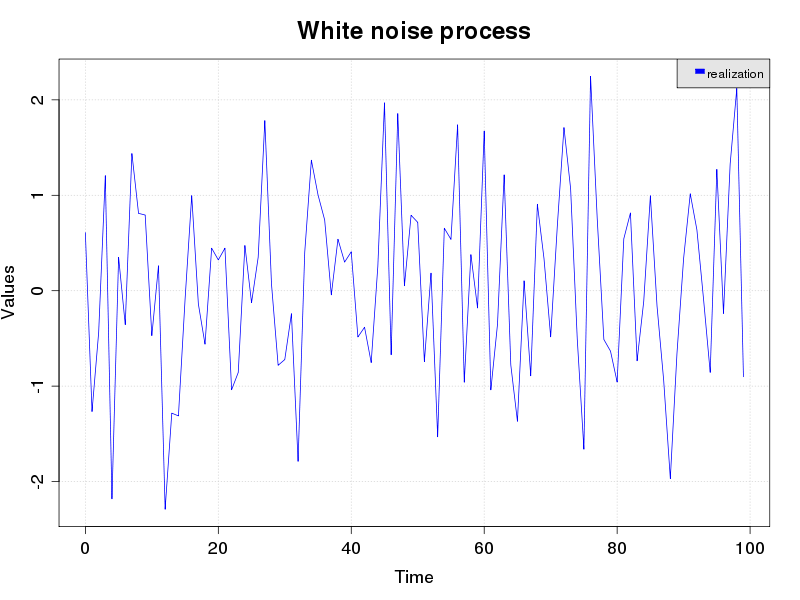
\includegraphics[width=7cm]{whitenoise_realization.png}
      \caption{Realization of a white noise with distribution $\mathcal{N}(0, 1)$}
      \label{whitenoise_Realization}
    \end{center}
  \end{minipage}
  \hfill
  \begin{minipage}{9cm}
    \begin{center}
      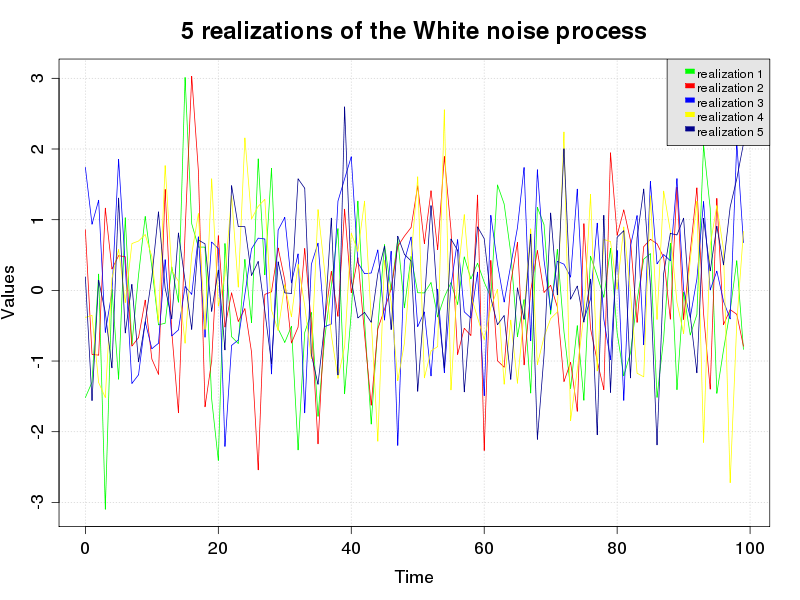
\includegraphics[width=7cm]{whitenoise_realizations.png}
      \caption{5 realizations of a white noise with distribution $\mathcal{N}(0, 1)$}
      \label{whitenoise_Realizations}
    \end{center}
  \end{minipage}
\end{figure}


